\section{Blobs and holes}
%
The aim of this chapter is to characterize the intermittent structures observed in the time traces in \cref{fig:combinedPlots008} by using a conditional averaging (CA) technique.
It turns out that the intermittent structures shares characteristics with what has been described as blobs in the literature.
We will here use the definition of a blob given in the review paper by D'Ippolito et. al. \cite{DIppolito2011}.
In this definition, a blob is a structure which satisfies the following properties:
%
\begin{quote}
    \begin{enumerate}[noitemsep]
            \item  it has a monopole (single-peaked) density distribution with a peak value much higher than the surrounding rms fluctuations of the background plasma (typically $\geq 2-3$ times higher);
            \item  it is aligned parallel to the magnetic field $B$ and its variation along $B$ is much weaker than in the transverse direction, i.e., $\delta/L_\|\ll1$;
            \item it has a dominant convective $\ve{E}\times\ve{B}$ velocity component in the direction of a charge-polarizing force, and an associated potential and vorticity with a dipole structure in the direction transverse to its propagation.
    \end{enumerate}
\end{quote}
%
Usually, the blobs observed in tokamaks are driven by magnetic field inhomogenities through the so-called grad-$B$ drift.
This drift is causing a polarization, and the polarization are driving the blobs outwards through the $\ve{E}\times\ve{B}$ drift.
The blobs in tokamaks are therefore self-propelled, and does not depend on local gradients of the plasma \cite{Krasheninnikov2008}.

\subsection{The conditionally averaging technique}
%
The CA technique is often used to tell something about the average of coherent structures in turbulence.
It has it roots in fluid dynamics \cite{Kovasznay1970}, with the first application to plasma physics in \cite{Huld1990}. Although improvements to the original technique has been done for for example noisy data recorded with a probe \cite{Teliban2007}, we will use the simple, classic variant of the technique here:
%
\begin{algorithm}
\begin{enumerate}[noitemsep,nolistsep]
    \item Record a signal in a single point over time.
    \item Set a threshold condition.
    \item When the signal reaches the condition, record a sub-signal $\tau$ time units before and $\tau$ time units after.
        The recorded sub-signal will be one of the samples in the conditional averaging.
    \item Take the average of all the samples, i.e. the recorded sub-samples.
\end{enumerate}
\end{algorithm}
%
Here, we will set the threshold condition on the radial flux.
Alternatively, we could have set a condition on the perturbation in $n$ itself.
This would have the disadvantage of including samples of perturbation which arises from poloidal rotation of a slightly elongated plasma.
In the end we are interested in structures which "has a dominant convective $\ve{E}\times\ve{B}$ velocity component" from point $3$ in the definition above.

\subsection{The averaged structures}
The time trace of the radial flux, together with three different conditions are shown in \cref{fig:blobFluxTT}.
%
\begin{figure}[htb]
    \begin{center}
        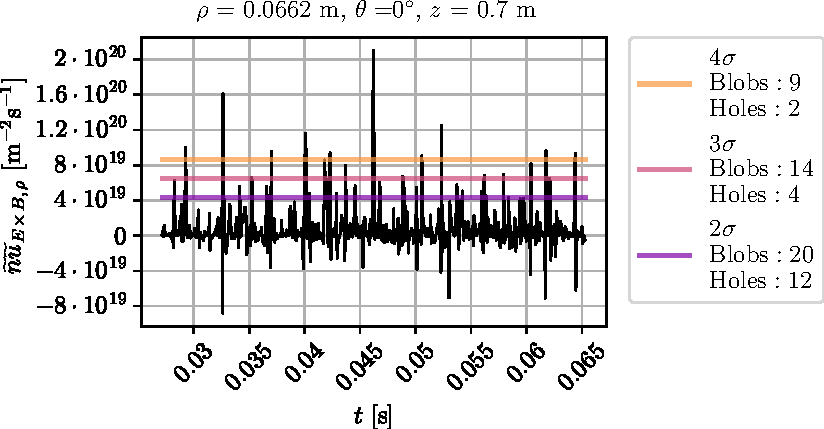
\includegraphics{fig/results/blobs/blobFluxTimeTrace_B0_008Tweak}
    \end{center}
    \caption{
        Time trace of the flux for $B=0.08\T$.
        The trigger conditions for $2\sigma$, $3\sigma$ and $4\sigma$ is indicated on the figure, and the number of events found are indicated in the legend.
    }
    \label{fig:blobFluxTT}
\end{figure}
%
Is apparent that the trigger signal is highly intermittent, as seen from the PDF in \cref{fig:blobFluxPDF}, which shows a skewness of approximately $3$, and an excess kurtosis of around $16.5$.
%
\begin{figure}[htb]
    \begin{center}
        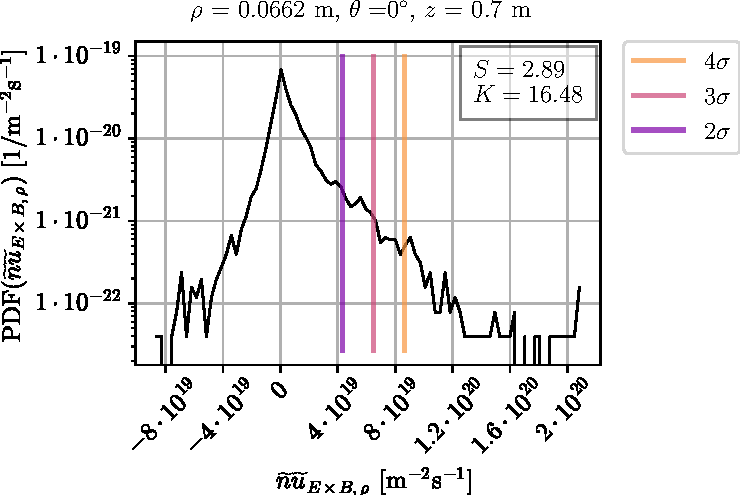
\includegraphics{fig/results/blobs/blobFluxPDF_B0_008Tweak}
    \end{center}
    \caption{
        The PDF of the radial flux from \cref{fig:blobFluxTT} ($B=0.08\T$), where $S$ indicates the skewness and $K$ the excess kurtosis.
    }
    \label{fig:blobFluxPDF}
\end{figure}
%
\Cref{fig:blobDensPDF} shows the PDF for the density signal at the same position.
We can observe that the density signal with its skewness around $1$ and an excess kurtosis of about $1.5$ is not as intermittent as the radial flux.
%
\begin{figure}[htb]
    \begin{center}
        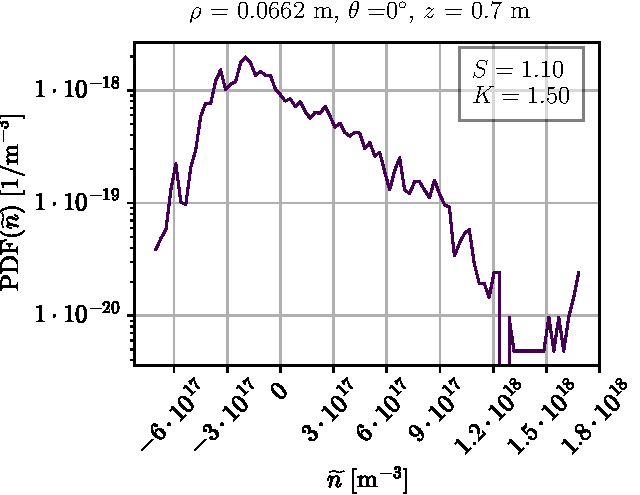
\includegraphics{fig/results/blobs/blobDensPDF_B0_008Tweak}
    \end{center}
    \caption{
        The PDF of the density, measured in the same point as \cref{fig:blobFluxPDF} ($B=0.08\T$).
        $S$ indicates the skewness and $K$ the excess kurtosis.
    }
    \label{fig:blobDensPDF}
\end{figure}
%

From \cref{fig:blobFluxTT}, we chose $\tau$ to be $4$ times the time of the maximum pulse duration (where the signal is above the threshold) of the flux.
We now have both the time where the condition is met and the time window set by $\tau$, and we can in principle use this to sample of any quantity in any spatial points.
In other words, we can use these time to conditionally sample the density $n$.
Before doing so, we note that we are dealing with two types of events, both giving a positive radial flux.
The events can either be:
%
\begin{enumerate}[noitemsep]
    \item A blob: A positive perturbation propagating in positive $\rho$.
    \item A hole: A negative perturbation propagating in negative $\rho$.
\end{enumerate}
%
The time trace of the CA structures are shown together in \cref{fig:blobAndHoleTT}.
%
\begin{figure}[htb]
    \begin{center}
        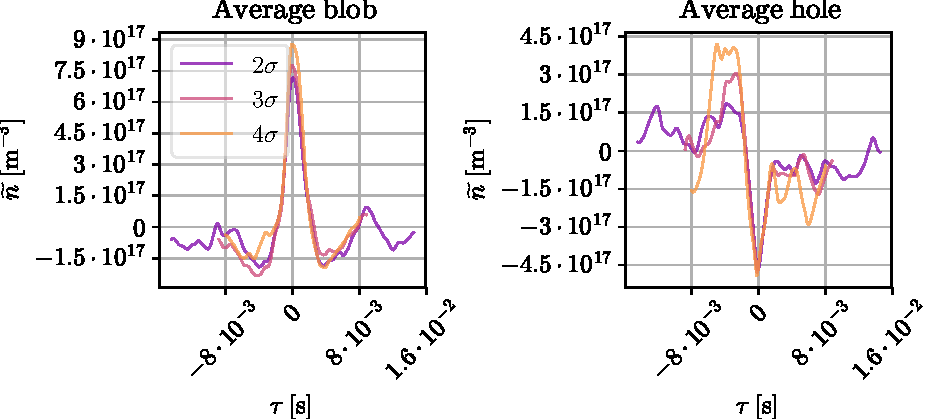
\includegraphics{fig/results/blobs/blobsAndHoles-B0_008Tweak}
    \end{center}
    \caption{The averaged blob and hole density structures for $\rho=0.0662\m,\;\phi=0^{\circ}\;z=0.7\m\;B_0=0.08\T$ found when using the trigger signal in \cref{fig:blobFluxTT}.}
    \label{fig:blobAndHoleTT}
\end{figure}
%
Note that the amplitude of the blobs and the holes are relatively insensitive to the choice of the condition.
This would not be the case in a truly random signal (i.e. Gaussian white noise), where lower amplitude events would decrease the CA amplitude for lower conditions.

Instead of sample the density at the same point as the condition is set, we can sample the whole perpendicular plane for the density fluctuations.
The result is shown in \cref{fig:perpBlob008}.
%
\begin{figure}[h!]
\begin{tabular}{ccc}
  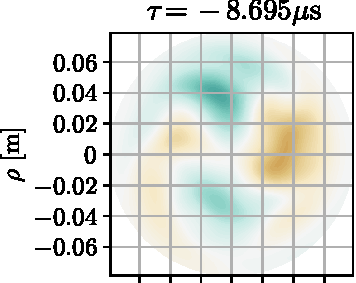
\includegraphics{fig/results/blobs/matrix-perp-blobs-B0_0.08-fluct/0} &
  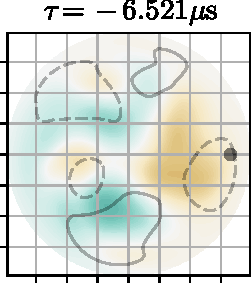
\includegraphics{fig/results/blobs/matrix-perp-blobs-B0_0.08-fluct/1} &
  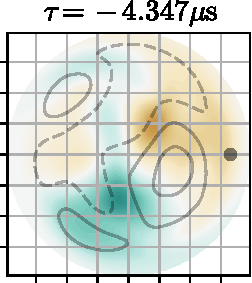
\includegraphics{fig/results/blobs/matrix-perp-blobs-B0_0.08-fluct/2} \\
  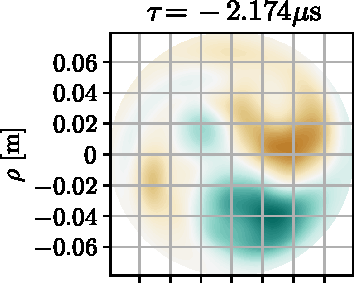
\includegraphics{fig/results/blobs/matrix-perp-blobs-B0_0.08-fluct/3} &
  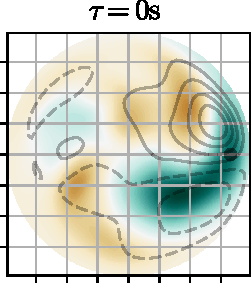
\includegraphics{fig/results/blobs/matrix-perp-blobs-B0_0.08-fluct/4} &
  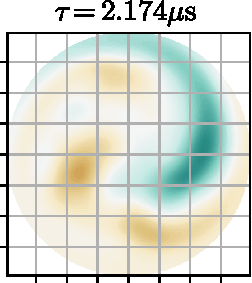
\includegraphics{fig/results/blobs/matrix-perp-blobs-B0_0.08-fluct/5} \\
  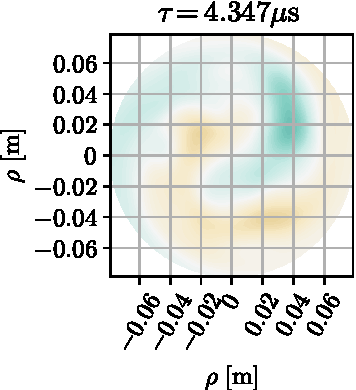
\includegraphics{fig/results/blobs/matrix-perp-blobs-B0_0.08-fluct/6} &
  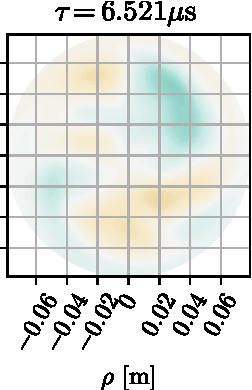
\includegraphics{fig/results/blobs/matrix-perp-blobs-B0_0.08-fluct/7} &
  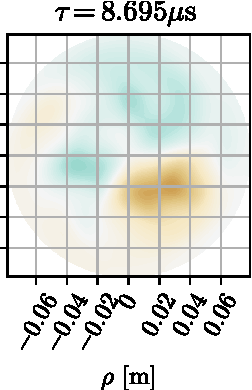
\includegraphics{fig/results/blobs/matrix-perp-blobs-B0_0.08-fluct/8} \\
  \multicolumn{3}{c}{\hspace*{2cm}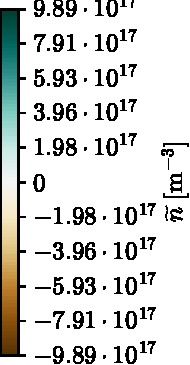
\includegraphics[angle=-90]{fig/results/blobs/matrix-perp-blobs-B0_0.08-fluct/colorbar}}
  \\
\end{tabular}
\caption{Perpendicular snapshot at $z=0.7\m$ showing the density fluctuations of the conditionally averaged field at $B=0.08\T$.}
\label{fig:perpBlob008}
\end{figure}
%
Although we are setting the condition at the flux at $\theta = 0$, we can see that the blob start to form around $\theta = 3/2 \pi$ in $\tau=-4.347\mu \s$.
This structure is then transported radially outwards, and starts to get sheared as soon as it reaches the region with high $\Om$ as indicated in \cref{fig:radProfs}.



\subsection{Waiting times and pulse width distribution}
%
Although we have few events
%
\footnote{
    More events can be made by running the simulations for longer time.
    The only limit is relatively long simulation times together with large data files.
}
%
, we would briefly indicate the trend of the waiting times and pulse width distribution.
A similar exercise is done in for example \cite{Hornung2011}, where it is found that the average temporal width of the pulse is a fraction of the period of a characteristic drift-wave, the peak of the waiting time PDF occurs approximately around one drift-wave period and the waiting time is much longer than a drift-wave period.
The waiting time and pulse widths in our case is shown in \cref{fig:tempStatBlob}.
As expected, the waiting time goes down the value of the triggering signal as more events are included in the sampling, and because the events will appear broader.
Because of this, also the pulse width goes up for decreasing value of the triggering signal.
%
\begin{figure}[h!]
    \begin{center}
        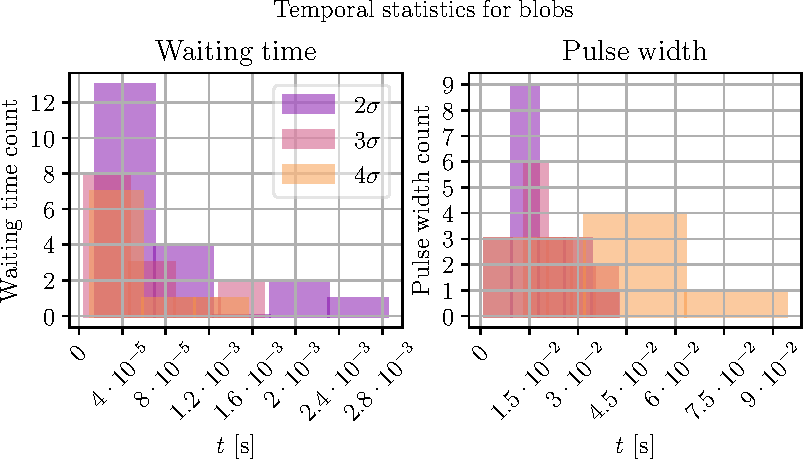
\includegraphics{fig/results/blobs/blobStatsB0_008Tweak}
    \end{center}
    \caption{
        Waiting times and pulse widths of $n$ for the conditional samples found for $B=0.08\T$.
    }
    \label{fig:tempStatBlob}
\end{figure}
